%------------------------------------------------
% test3.tex - test file for camel.cls
%------------------------------------------------
\documentclass{camel}
\usepackage{camel}
\usepackage{arholiad}
\academicyear{2014-15}
\modulecode{MAXXXX}
\moduletitle{Camel Theory}
\usepackage{lipsum}

%------------------------------------------------
\begin{document}

\chapter{Introduction}\label{ch:intro}

Hello, how's it going?
\begin{figure}
\centering
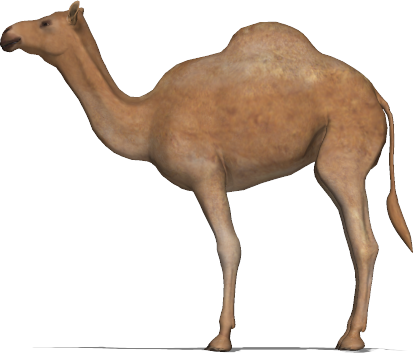
\includegraphics[scale=0.25]{humpty}
\caption{Humpty the Camel.}
\label{humpty-the-camel}
\end{figure}
No more figures.

\chapter{Background}\label{ch:background}

Initial text.
\begin{itemize}
\item First item of list
\begin{enumerate}
\item First item of nested list.
\item Second item of nested list.
\end{enumerate}
\item Second item of list
\end{itemize}
Final text.

\chapter{Labels, References and Citations}

\begin{itemize}
\item Here we include a label: \label{ch:introduction}.
\item Here we include a reference: \ref{ch:introduction}.
\item Here we include a citation: \cite{evans02}.
\end{itemize}

\chapter{Some exercises}\label{ch:exercises}

\begin{exercise}\label{ex:demo}
This is the introduction.
\begin{questions} 
\question This is the first question.\label{qu:first-question}
\begin{answer} 
This is an answer to the first question.
\end{answer} 
\question This is the second question.\label{qu:second-question}
\begin{answer} 
This is an answer to the second question.
\end{answer} 
\question This is the third question.\label{qu:third-question}
\begin{parts}
\part This is the first part of the third question
\begin{answer} 
This is an answer to the first part of the third question.
\end{answer} 
\part This is the second part of the third question
\begin{answer} 
This is an answer to the second part of the third question.
\end{answer} 
\end{parts}
\end{questions} 
\end{exercise}

\chapter{Some maths}
Let $\alpha$ and $\beta$ be ...
\[
\int_0^1 2x\,dx = 1. 
\]
Here is an equation with a label:
\begin{equation}\label{eq:einstein}
E = mc^2
\end{equation}



\end{document}

